\subsection{Unterschied Halbleiter vs Metalle \todo{0x}}\label{k2:metalle}
Metalle: Gute Leitf\"ahigkeit aufgrund des vorhandenen Elektronengas. Bereits mit wenig Energie werden genug Elektronen gel\"ost um zu leiten.\\
Halbleiter: Leitf\"ahigkeit liegt zwischen Leitern und Nichtleitern. (Bandl\"ucke $< 1eV$)\\
Nichtleiter (Bandl\"ucke $> 3eV$).\\
Siehe \Cref{fig:bandLHL}.
\begin{figure}[h]
        \centering
        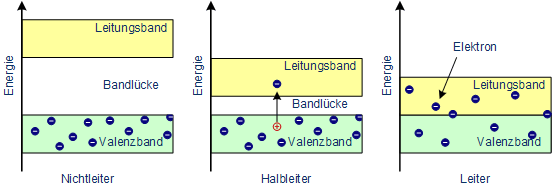
\includegraphics[width=0.6\textwidth]{fig/baendermodellLHL}
        \caption{B\"andermodell f\"ur Nichtleiter, Halbleiter und Leiter}
        \label{fig:bandLHL}
\end{figure}

\subsection{Grund für die Bildung von Festkörpern \todo{1x}}\label{k2:festkorper}
Ausgang: Wasserstoffatom als Modellsubstanz. Hier gillt eine sph\"arische Wellenfunktion:
\begin{equation}
    \Psi_H(r) = C \cdot e^{(-\frac{r}{a_0})}
\end{equation}
mit $a_0$ Bohr'scher Radius.\\
Daraus wird ein 2D-Gitter aus Automen gebaut, wobei davon ausgegangen wird dass Bindungen nur zwischen n\"achsten Nachbaren auftritt (tight binding Methode).
Die Energieskala wird so gew\"ahlt, dass der Zustand des neutralen Atoms (das Elektron befindet sich direkt am Atom) dem Energienullpunkt entspricht.\\
Gibt man einen weiteren Wasserstoffkern dazu, kann sich das Elektron entweder so positionieren, dass es beide Potentiale sp\"urt (seine Energie wird abgesenkt, $\Psi_1$, bindender Zustand) oder so, dass es sich nur bei den Ionen aufhält (seine Energie wird angehoben, $\Psi_2$, anti-bindender-Zustand).
\begin{center}
    \begin{align*}
        \Psi_1 &= \Psi_H(r_1)+\Psi_H(r_2)\\
        \Psi_2 &= \Psi_H(r_1)-\Psi_H(r_2)
    \end{align*}
\end{center}
\begin{figure}[h]
        \centering
        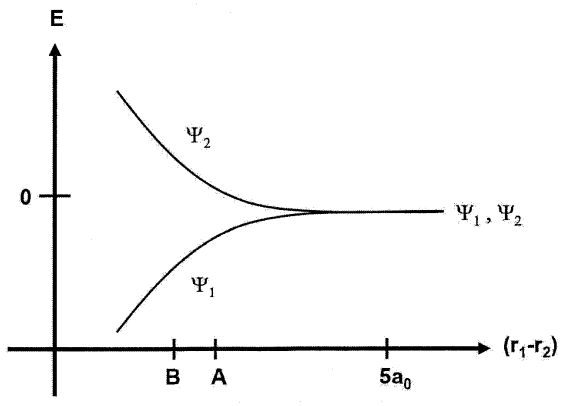
\includegraphics[width=0.6\textwidth]{fig/atomdistanz}
        \caption{Energie des bindenden- und anti-bindenden Zustands in Abh\"angigkeit vom Abstand der Atome. A = metall, B = halbleiter}
        \label{fig:atomdistanz}
\end{figure}
\subsection{Leitungsband, Valenzband, Ef aufzeichnen \todo{2x}}\label{k2:leitungsBand}

Siehe \Cref{fig:bandLHL}. Ef?

\subsection{Kroning Penny Modell \todo{0x}}\label{k2:kroningpenny}
Vereinfachtes Modell für Elektronen in Kristallgitter, verwendet ein einfaches periodisches Kristallpotenzial \autoref{fig:kronig-penney} ($a_0$ ist die Gitterkonstante)

\begin{equation}
    V(x + a_0) = V(x)
\end{equation}

\begin{figure}
    \centering
    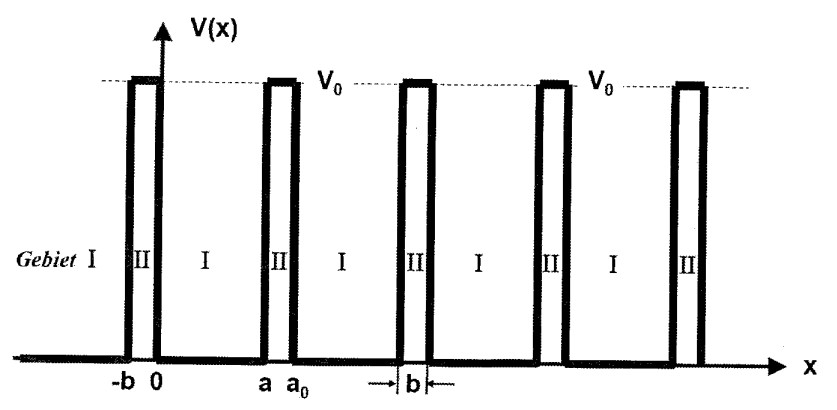
\includegraphics[width=0.66\textwidth]{fig/kronig-penny.jpg}
    \caption{Eindimensionales Kronig-Penney-Potenzial}
    \label{fig:kronig-penney}
\end{figure}

und vernachlässigt alle anderen Wechselwirkungen. Die Wellenfunktion der Elektronen sind Bloch-Funktionen.
Eine \textit{Bloch-Welle} (\autoref{fig:h-wave}) ist eine spezielle Wellenfunktion. Sie wird durch eine einfache planare Welle die mit einer periodische Funktion moduliert wird beschrieben.
Das schaut dann so aus:
\begin{equation}
    \Psi(r) = e^{i\cdot k\cdot r}\cdot u(r)
\end{equation}

\begin{figure}
    \centering
    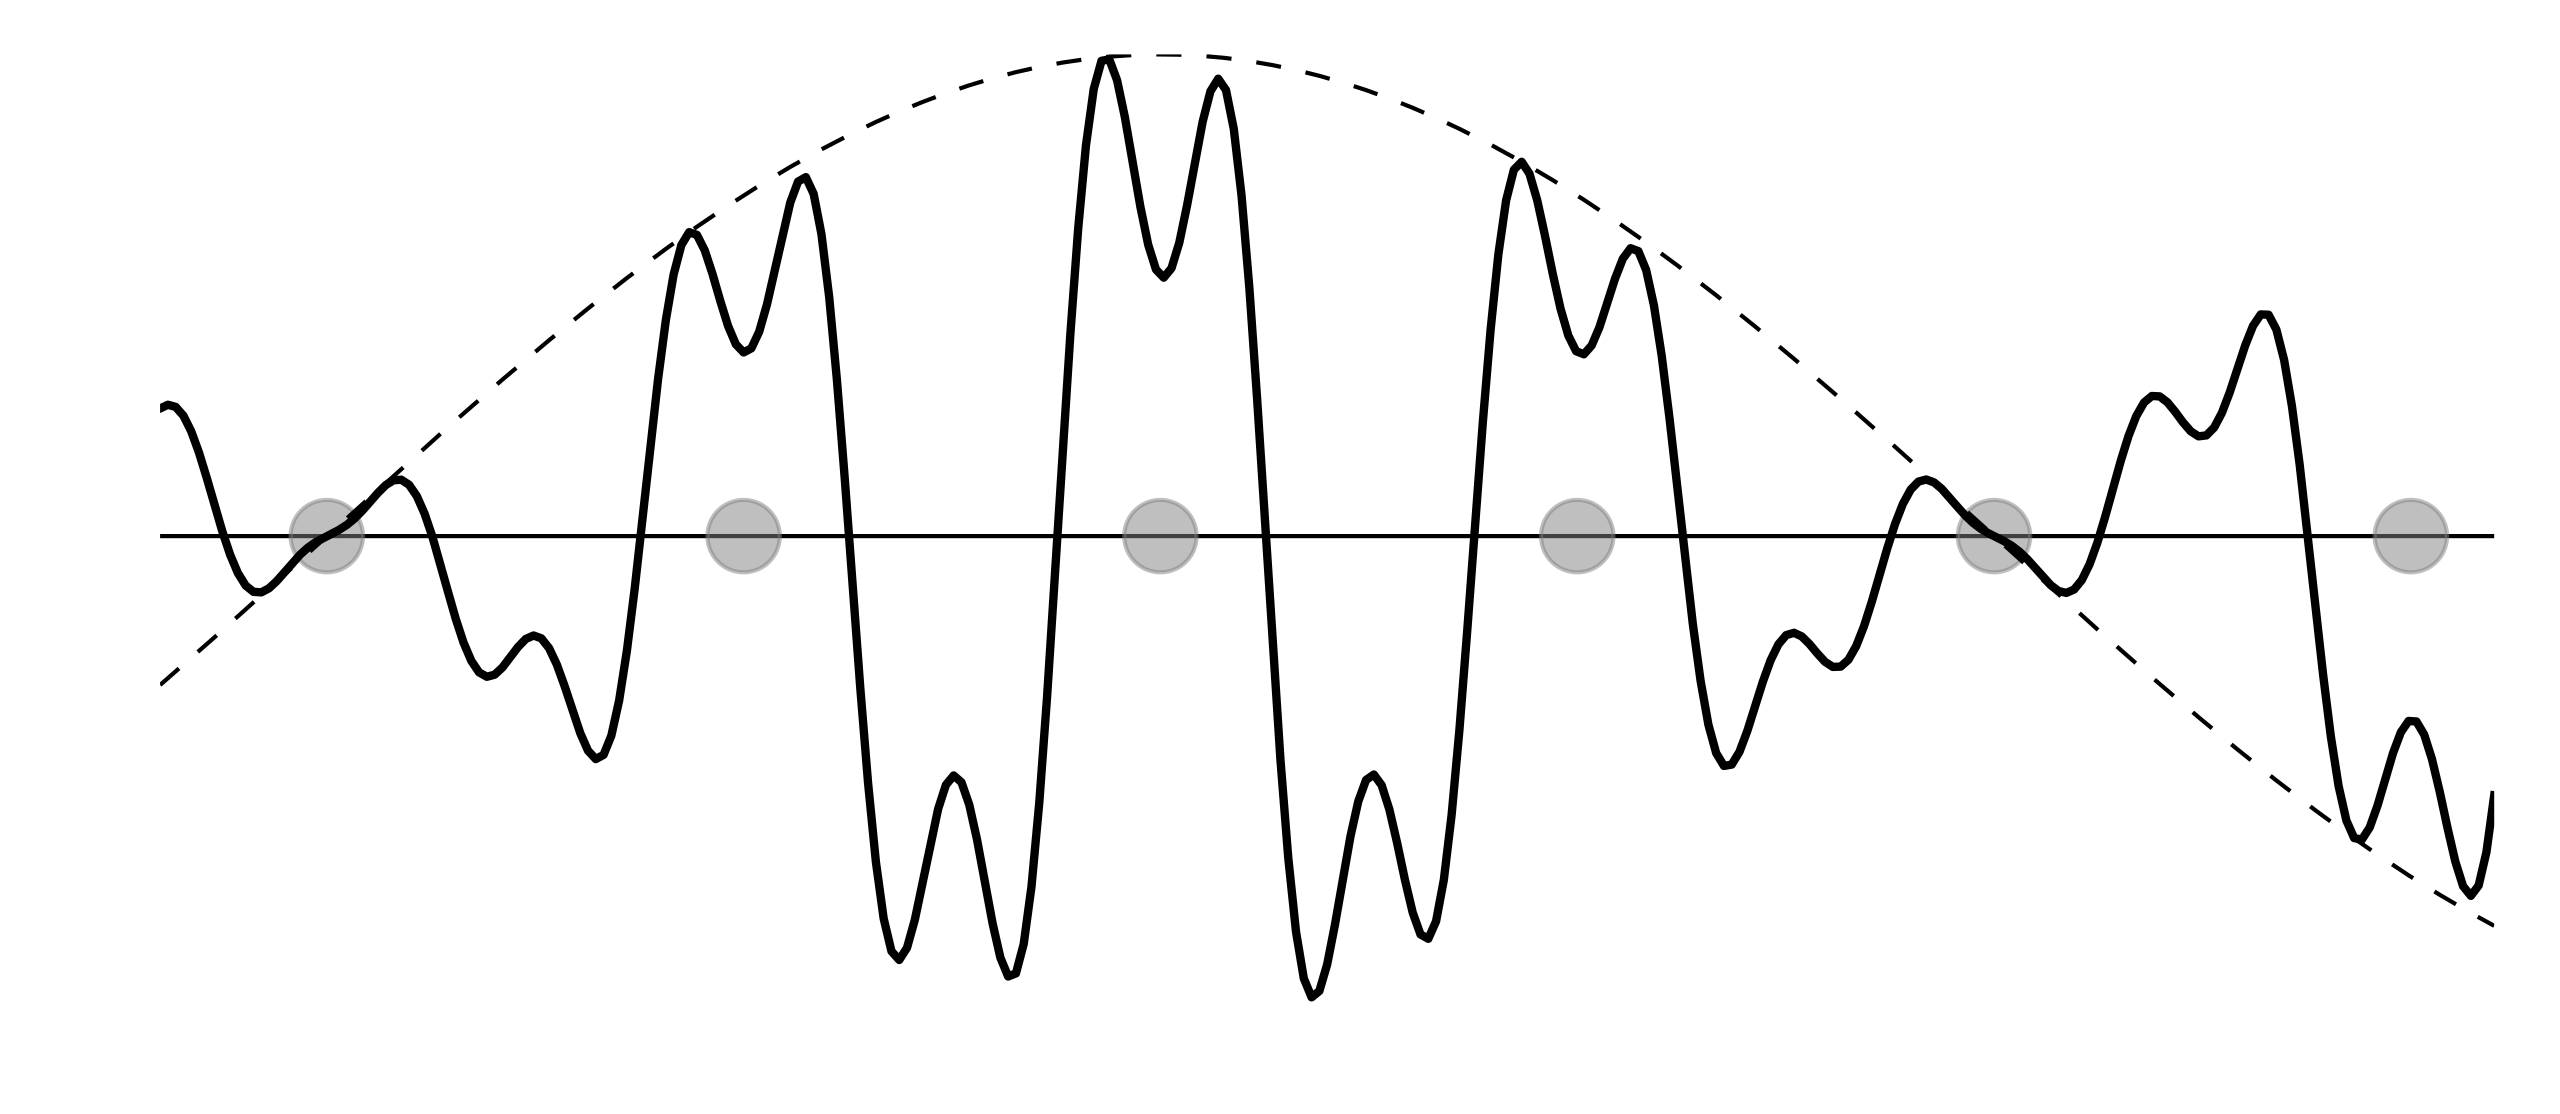
\includegraphics[width=0.66\textwidth]{fig/bloch-wave}
    \caption{Solid line: A schematic of a typical Bloch wave in one dimension. (The actual wave is complex; this is the real part.) The dotted line is from the $e^{ikr}$ factor. The light circles represent atoms.}
    \label{fig:h-wave}
\end{figure}

\begin{enumerate}
    \item $r$ ... Position
    \item $u$ ... periodische Funktion mit der selben periodizität wie das Kristallgitter
    \item $k$ ... Wellenvektor
\end{enumerate}

Herleitung für das eindimensionale Problem über periodische Kette von Rechteckbarrieren. Darüber kann man dann die Schrödinger Gleichung lösen, der Ansatz dafür ist folgender: $\Psi_k(x) = u_k(x)\cdot e^{ikx}$, wobei $u(x) = u(x+a+b)$ (Blochfunktion).

Man kann das Modell dann weiter vereinfachen (Breite Potenzialbarrieren gegen 0, Barrierenwirkung aber gleich) und es ergibt sich eine Bestimmungsgleichung  für die erlaubten Energiebänder für eine bestimmte Barrierestärke $P = \frac{ma}{\hbar^2} \cdot V_0 \cdot b$.

Die Bestimmungsgleichung selbst sieht so aus: 

\begin{equation}
    P\frac{sin(\alpha a)}{\alpha a} + cos(\alpha a) = cos(ka)
\end{equation}

Die Bestimmungsgleichung (auch Eigenwertgleichung) für die erlaubten Energiebänder enthält jetzt nur mehr die folgenden Paramter:

\begin{enumerate}
    \item P ... Barrierenstärke
    \item a ... Gitterkonstante (der Abstand zweier benachbarter Gitterelemente)
    \item $\alpha$ ... Indirekt die Energie
\end{enumerate}

\subsubsection{Grafische Lösung}
\begin{figure}
    \centering
    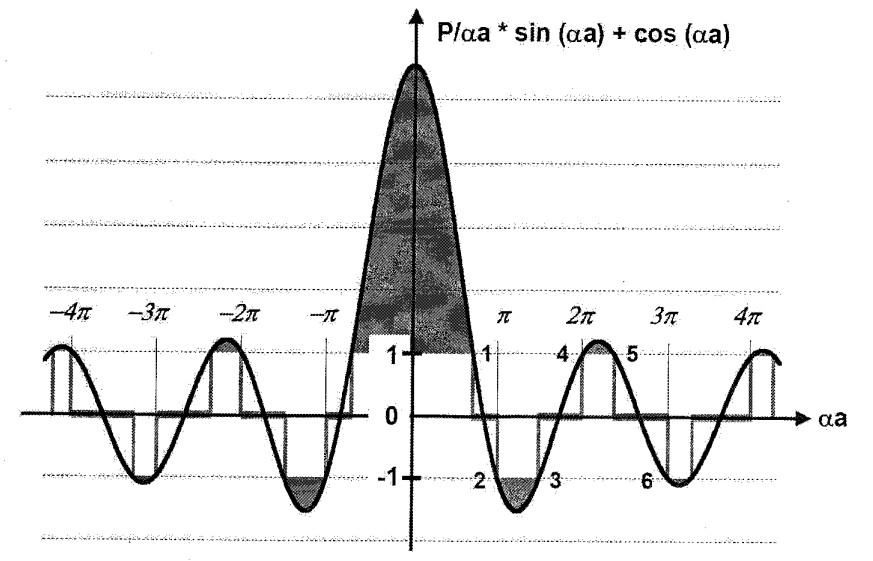
\includegraphics[width=0.66\textwidth]{fig/krong-penney-grafisch.jpg}
    \caption{Graphische Lösung des Kronig-Penney-Modells}
    \label{fig:kronig-penney-grafisch}
\end{figure}



Erkl\"aren, Skizzen, Rechenvorgang, grafische L\"osung, Herleitung e(k) Diagramm

\subsection{Entstehung der Halbleiter \todo{0x}}\label{k2:entstehungHalbleiter}

Verschiebt man die inneren Atome einer periodischen atomaren Anordnung so, dass der Abstand eines Paares kleiner wird als der Abstand der anderen Atome, \"andert sich die Verteilung der Energieniveaus. Die Bindungsenergie des n\"aheren Paares steigt, der Abstand zwischen bindendem und anti-bindendem Zustand wird wesentlich gr\"o{\ss}er. F\"ugt man weitere Atome hinzu, belibt der gr\"o{
\ss}ere Energieabstand erhalten. Die weiteren Energieniveaus gruppieren sich um die bindende und anti-bindende Energie (\Cref{fig:energieHalbleiter}).

\begin{figure}[h]
        \centering
        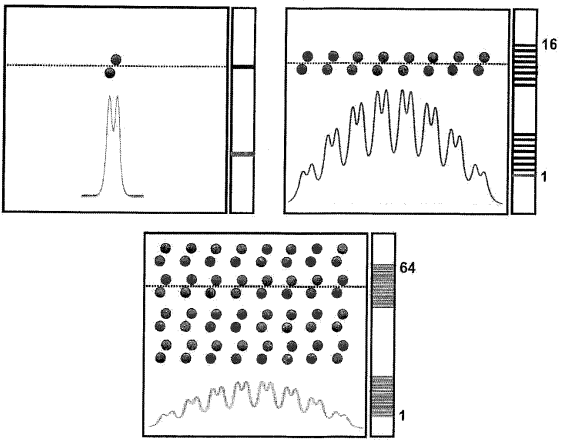
\includegraphics[width=0.6\textwidth]{fig/energieHalbleiter}
        \caption{Energiegruppierung in Halbleitern}
        \label{fig:energieHalbleiter}
\end{figure}

Es entstehen immer dann Halbleiter, wenn sowohl k\"urzere als auch l\"angere Bindungsl\"angen existieren. Erreichen kann man das z.B. durch inneinanderstellen von zwei Gittern (\Cref{fig:gitterstrukturen}).

\begin{figure}[h]
        \centering
        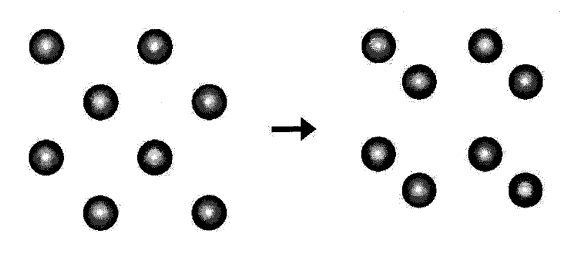
\includegraphics[width=0.6\textwidth]{fig/gitterstrukturen}
        \caption{Anordnung des zweidimensionalen Gitters}
        \label{fig:gitterstrukturen}
\end{figure}

Auf Grund der st\"arkeren Bindungen sind Halbleiter h\"arter als Metalle. Bei $T=0K$ haben sie keine Leitf\"ahigkeit.
Das untere Band (Name Valenzband) ist vollständig mit Elektronen besetzt, das obere Band (Leitungsband) ist leer.
Es gibt gleich viele Zustände im unteren und oberen Band. Wenn Ladungsträger ins obere Band angeregt werden, können
sie sich frei bewegen und führen zu einer hohen Leitfähigkeit.

\subsection{Phononen \todo{0x}}\label{k2:phononen}
F\"ur zwischenatomare Kr\"afte kann ein lineares Kraftgesetzt angenommen werden. Die Gitterschwingungen sind dann harmonische Oszillatoren mit quantisierter Energie $(n+\frac{1}{2}\hbar \omega)$.
Weil die m\"oglichen Energieniveaus einer Schwingung den gleichen Abstand $\hbar \omega$ besitzen, k\"onnen die Gitterschwingungen (analog zu den Photonen im elektrischen Feld) als teilchen gesehen werden, diese werden Phononen genannt. Sie geh\"oren zu den Bosonen.

\begin{table}[H]
    \centering
    \begin{tabular}{rcc}
         & Elektron & Phonon \\
         Ausbreitungsvektor & $\vec{k}$ & $\vec{q}$ \\
         Impuls & $\vec{p} = \hbar \cdot \vec{k}$ & $\vec{p} = \hbar \cdot \vec{q}$ 
    \end{tabular}
\end{table}

Bei Phononen spricht man vom Kristallimpuls, der nicht der Schwingung der Atome entspricht.\\
Die Zahl der im Mittel angeregten Phononen ist durch die Bose-Einstein Beziehung gegeben:
\begin{equation}
    n = \frac{1}{e^{\frac{\hbar\omega}{k_B T}}-1}
\end{equation}